% old document class in draft mode: \documentclass[a4paper,titlepage,draft]{article}
\documentclass[a4paper,titlepage]{article}

% Page size
%\usepackage{a4wide}

% Fonts and Language Support
\usepackage[utf8]{inputenc} 
\usepackage[T1]{fontenc}
\usepackage{mathptmx}

% Other packages\\

\usepackage{setspace}
\usepackage{fancyhdr}
\usepackage{fixme}
\usepackage{graphicx}
\usepackage{float}
\usepackage{listings}
\usepackage{underscore}
\usepackage{lastpage}
\usepackage{pdfpages}
\usepackage{tocvsec2}
\usepackage{verbatim}
\usepackage[bookmarks]{hyperref}

% Macros
\newcommand{\HRule}{\rule{\linewidth}{0.5mm}}
\newcommand{\SYSNAME}{RentIt}

% Style setup
\setlength{\headheight}{15pt}
\pagestyle{fancyplain}
%\cfoot{\thepage\ of \pageref{LastPage}}
%\setstretch{1.15}

% Header and footer
\lhead{}
\rfoot{\fancyplain{}{\thepage \hspace{1pt} of \pageref{LastPage}}}
\cfoot{}

%%%%%%%%%%%%%%%%%%%%%%%%%%%%%%%%%%%%%%%%%%%%%%%%%%%%%%%%%%%%%%%%%%%%%%
% Frontpage
\begin{document}

% diverse
\parindent=0pt % Ingen indrykkning
\parskip=8pt plus 2pt minus 4pt

% front page
\title{Second Year Project: Software Development in Large Teams with International Collaboration\\-\\Moofy}
\author{Kristian Brink Gansted\\ \emph{kbri@itu.dk}
    \and Niclas Benjamin Tollstorff\\ \emph{nben@itu.dk}
    \and Niels Lijledahl Christensen\\ \emph{nlch@itu.dk}
    \and Niels Roesen Abildgaard\\ \emph{nroe@itu.dk}
    \and Sigurt Bladt Dinesen\\ \emph{sidi@itu.dk}}

\maketitle

% Start on page 0
\setcounter{page}{1}

% TOC
\tableofcontents
\newpage

% Body
%\onehalfspace
\begin{spacing}{1.15}
%%%%%%%%%%%%%%%%%%%%%%%%%%%%%%%%%%%%%%%%%%%%%%%%%%%%%%%%%%%%%%%%%%%%%%
\section{Introduction}

This report is written by a team of five students at the IT-University of Copenhagen (ITU)
studying Software Development on second year (4th semester).

The authors of this report are Niclas Benjamin Tollstorff (nben@itu.dk), Niels Liljedal
Christensen (nlch@itu.dk), Sigurt Bladt Dinesen (sidi@itu.dk), Kristian Brink Gansted
(kbri@itu.dk), and Niels Roesen Abildgaard (nroe@itu.dk).

The project used as a basis for this report was done in collaboration with a group of
students from the Singapore Management University (SMU), and had the goal to develop an
application that would allow users to buy and rent films and music. The application consisted
of a server developed by the ITU students and a browser-based client developed by the SMU
students.

The Singaporean team was made up of Chai Ching Hsiang Robert, Tan Kah How Kelvin, and
Chong Wen Xiong Nick.

As a part of the course \emph{System Development and Project Organisation}, we have learned
about several tools and methods to use in a software development context.

The basis for these methods is the book \emph{Project Management for Information Systems}
(5th edition) by James Cadle and Donald Yeates, which explains these methods as well
as which situations they may be used in.

We will detail project management methods used during our project, and problems that may arise
when using these. In the form of a case study, this report looks into modifications to the
methods used, and how these modifications help the project. Issues that arose during the project
are listed and paired with the methods we used to overcome them.

Finally we will analyze the effectiveness of all the methods used with an aim to determine
the usefulness of each method. The analysis is based on the team’s experiences with the
methods and is purely qualitative.

Throughout the report, we will describe and discuss our experiences with:

\begin{itemize}
    \item risk management through \emph{risk analysis}, as well as actual handling of risks
        (Sections \ref{sec:EmpiriRiskManagement} \& \ref{sec:AnalysisRiskManagement});
    \item project planning through \emph{work breakdown structure} and \emph{identification of
        dependencies}, resulting in a plan in the form of a Gantt diagram (Sections
        \ref{sec:EmpiriPlanning} \& \ref{sec:AnalysisPlanning});
    \item estimation of features through \emph{planning poker} (Sections
        \ref{sec:EmpiriEstimation} \& \ref{sec:AnalysisEstimation});
    \item choice of development framework (or methodology) for a small project (Sections
        \ref{sec:EmpiriOrganizational} \& \ref{sec:AnalysisOrganizational});
    \item quality control, using a \emph{quality plan} (Sections \ref{sec:EmpiriQualityControl}
        \& \ref{sec:AnalysisQualityControl}); and
    \item progress monitoring, keeping in mind the initial planning and estimation (Sections
        \ref{sec:EmpiriProgress} \& \ref{sec:AnalysisProgress}).
\end{itemize}
\pagebreak
\section{Business Case}
The following section aims to provide intuition to our decision processes, by
giving a brief introduction to our business case.

\subsection{Business opportunity}
With this project we want to address the problem of piracy in the digital-media
industry. Piracy is an often committed illegal activity, with recent research
showing that around 30\% of 15-29 year-olds (in Denmark) engage in piracy of
movies and tv-shows\cite{pirates}. The same study showed that most pirates
would prefer to acquire their media in legal ways, but that current options
lack the high accessibility that piracy offers.

Based on the study mentioned above, we believe that we can address the problem
of piracy by providing an accessible way for customers to acquire media
legally.

Rather than making an ad-hoc streaming service, we aim to broaden the client
range by generalising the concepts of online media rental and purchase into a
centralized service, and letting third-party developers use that as a backbone
for their own rental/purchase services.

\subsection{Concept elaborated}
We aim to provide a service which allows users to buy and rent movies and
songs. Upon purchase, the user will be able to both stream and download the
media directly from our service, as accessibility is a key quality in the
service.

We hope to convert media pirates, who want to acquire media in a legal manner,
but simply lack the means to do so. This is to be achieved through accessible,
DRM-free media. Since media streaming is popular\cite{ott} we do not wish to
restrict ourselves to this segment, as we believe a typical family will have
interest in our service too.

While big brands already exist in the media streaming industry (e.g. NetFlix
for movies/series, or Spotify for music) our concept differs in certain ways,
as detailed below:

\begin{itemize}
    \item We keep both movies and media gathered in one single service. We believe that, 
        in the upcoming era of smart tvs and media centers \cite{smarttv}, it will be
        desirable to have media stored in one application rather than having several
        different apps on a single media center.
    \item We do not use the \emph{Recurring Revenue model (Subscription
	model)}\cite{businessmodel}. Our users are not limited by a
	subscription period in which they can access their media. Instead,
	a bought item will be treated as their property, free for download
	or streaming at any time, thus providing high accessibility. In
	addition, recent research\cite{ott} has predicted that subscription
	services will not dominate in the future, while other forms of
	digital content distribution will.
\end{itemize}

\subsection{Impacts and risks}
This section will elaborate on the immediate risks associated with the concept.
Since streaming services have been around for several years the technology
needed has matured, and as such we have few risks associated with the
technological aspects. The technology risk with the largest impact on the
business, is that we cannot find a fullfilling security mechanism for the
downloaded files, making them shareable without copyright concerns. Note that
we have found feasibility tests of this mechanism to be outside of the scope of
this report.

The other risks, with large impact, are external factors:
\begin{itemize}
\item A solid customer base may not be achieved.
\item A partnership with content providers may not be achieved.
\end{itemize}

These risks are mostly concerned with marketing, and strategies to avoid them
is considered out of scope for this report.

\section{Analysis and Design}
\subsection{Requirements}
\label{sec:requirements}
As part of the analysis, we need a set of requirements for our product to
establish what users will and will not be able to do with the system. This
section describes and discusses our choice of requirements and use cases.

We did not immediately arrive at our current requirements. They have changed
over a series of iterations in which we revised and discussed them internally in
the group, as well as with the Singaporean team. For example, our first draft of
requirements did not include songs at all. It was not until the Singaporean team
told us that they were required by their professor to include songs in their
service that this became part of our requirements. The Singaporean team also
made the suggestion that media files should include ratings and view count to allow us to
sort by rating and popularity. In general, the requirements were almost
exclusively changed on request from the Singaporean team.

There are two types of primary actors: users and managers. A manager’s rights
are a superset of a regular user's. 

In the following requirements document, the word \emph{user} refers to an
existing, registered user. Artifact shall refer to a movie or song (the
products available for rent/purchase in the system). For the sake of this
description, the artifact properties are divided into two categories:
\emph{intrinsic} or \emph{extrinsic} to the artifact.

\emph{Intrinsic}
properties are those describing the artifact. Examples are title, URI to image,
and average rating. These properties are decided by the system actors, and are
not necessarily present. A manager may choose not to include an image URI, and
new artifacts may have no ratings.

\emph{Extrinsic} parameters are those
describing the artifacts from the system's perspective. Examples are id, and
view count. These parameters are completely determined by the system, and are
present regardless of actor interaction.

\textbf{Artifacts:}
\begin{enumerate}
\item A movie must have intrinsic properties describing its title, year of
	release, director(s), and genre(s).
\item A song must have intrinsic properties describing its title, year of
	release, artist(s), album title, and genre(s).
\item An artifact must have an extrinsic property describing its unique id.
\item An artifact must have an intrinsic property to describe an URI pointing to
	an image (E.g. cover image for movies).
\item An artifact must have a property to describe its average
	user-rating. This property is intrinsic (determined by actors, may be
	non-present) but only individual ratings are set by by actors, the
	average is maintained by the system, and it must not be an option for an
	actor to edit the average directly.
\item An artifact must have an intrinsic property for a textual description.
\item An artifact must have a property to describe both a purchase price, and a
	rental price. These are intrinsic (determined by the actors) but their
	presence must be enforced by the system. \label{itm:priceReq}
\item An artifact must have properties to describe its view count. I.e. number
	if times the artifact has been viewed or downloaded.
\newcounter{enumTemp}
\setcounter{enumTemp}{\theenumi}
\end{enumerate}

\textbf{Users:}
\begin{enumerate}
\setcounter{enumi}{\theenumTemp}
\item A (non) user must be able to register an account.
\item A user must be able to login to her account.
\item A user must be able to edit her account.
\item A user must be able to close her account.
\item A previous user must be able to reopen her closed account.
\item A user may deposit money into her account, to be used for later
	purchases.
\item A user must be able to purchase an artifact, which will then be associated
	with her account, for as long as the artifact is available on the
	service.
\item A user must be able to rent a artifact, which will then be associated
	with her account for 2 days.
\item A user must be able rate any artifact.
\item A user must be able to change her rating of any artifact.
	This cannot be registered as a new rating, but must be an alteration of
	the old one, so that a user can only give the same artifact \emph{one}
	rating.
\item A user must be able to overview artifacts, sorted by the following
	criteria: lexicographic, release date, genre, rating, and
	popularity (per view count).
\item A user must be able to locate a specific artifact through text search,
	listing artifacts where any property matches the search string.
\item A user must be able to watch any artifact associated with her account
	in the browser, as long as it is still available through the service.
\item A user must be able to download any artifact associated with her account,
	as long as it is still available through the service.
\item A user must be able to retrieve a listing of any artifact that is, or has
	been, associated with her account, as long it is still available through
	the service.
\item A user must be able to find all artifacts that are currently associated
	with her account, as long it is still available through the service (I.e.
	artifacts that are available to the user at the given time).
\setcounter{enumTemp}{\theenumi}
\end{enumerate}
\textbf{Managers:}
\begin{enumerate}
\setcounter{enumi}{\theenumTemp}
\item A manager's rights extend those of the user, so that a manager can do
	everything the user can, albeit without purchase.
\item A manager must be able to upload movies/songs
\item A manager must be able to create and edit the properties of any artifact,
	except for the \emph{extrinsic} properties; average rating and view
	count.
\item A manager must be able to delete movies/songs from the service.
\end{enumerate}

\subsubsection{Security and other Design Decisions}

When deciding on the
requirements for the system, several criteria are considered, and some
requirements which might be crucial in a real-life product are left out. These
decisions are mainly made on the basis that this is an educational project,
making these requirements more or less irrelevant to the project:
\begin{itemize}
\item We decided to leave out user authentication in our web services, so given
	the URL, anyone can download a movie our song without authenticating.
	The data structure does, however, support user authentication with each
	user having a password.
\item In a real-life renting service such as iTunes, once a user starts playing
	the movie that she has just rented, the movie will only be available
	for viewing in the next 48 hours. When a user rents and downloads a
	movie or song using our service, they can keep the file for as long as
	they want. However, the file is only available for download for a
	limited period of time.
\item Real-money payment is not implemented. Rather, a "fake" balance where
	people can deposit money to their account, for use when purchasing or
	renting movies and songs. However, given access to an E-commerce
	system, real-money payments could easily be implemented on top of his
	structure.
\end{itemize}

Notably, the web service and its clients have been developed separately.
Therefore, the requirements have become a conjunction of the SMU- and
SWU-clients' requirements, through which the web service's requirements are
implicitly described.

This sort of implicit requirements specification might not be recomendable, but
in this case the requirements were simple enough that it did not cause any real
trouble. However, care had to be taken when determining which requirements to
handle in the client, and which to handle in the API. Surprisingly, the SMU
client/SWU client situation somewhat simplified the issue. Having two
unrelated clients to the service, the web service interface came to be seen as a
general API, rather than a one-off, like the clients.
This view of the web service, made it an obvious choice to place
limiting requirements in the clients, and leave the service as flexible as
possible.

\textbf{For example... req 25}

\subsection{Deciding on the External API Form}

The two teams quickly agreed on using a RESTful JSON-based API as interface between
frontend (client) and backend (server). This still left a lot to design.

When designing an API it is important for it to be intuitive and attractive, as this
allows third-party developers, as well as our overseas colleagues, to use the API for
their purposes. Third-party developers in general represent a huge business opportunity
in our case, as the system requires purchases in order to actually access artifacts. This
means that third-party clients may create new revenue sources for us.

When discussing how to best attack the problem of what a \emph{nice API} is, we found two
options.

Either we could let the API handle arbitrary datatypes or have specific services for
every allowed datatype. The difference between the two possibilities can be illustrated
through which services are offered by them:

\begin{table}[hbt]
    \centering
    \begin{tabular}{ | l | l | l | }
        \hline
        \textbf{Abstraction level} & High abstraction & Low abstraction \\
        \hline
        \textbf{Services provided} & files/ & movies/ \\
        &  & songs/ \\
        \hline
    \end{tabular}
    \caption{Services offered by different abstraction levels}
\end{table}

In the high abstraction case a call to the files service may return any of the supported
data types, so the client can not know this for sure at the time of calling the service.
This problem can be solved in the following ways: first off, the client discovers content
through a service that will also disclose the type of the content (so it is already aware
of the type) and, secondly, the files-service itself will return the type of the content
as well as the content itself.

In contrast, the movies- and songs-services always return movies and songs, respectively.

This difference can be illustrated by looking at the services as if they were method calls.
In this case, the files-service would have a return-type of "Object", whereas the movies-
and songs-services would have "Movie" and "Song".

The high abstraction level works like a dynamically typed language (PHP, Javascript) would
work, wheras the low abstraction level works like a type-strong language like C\# or Java.

\subsubsection{Cost of Change}
In the high abstraction level service it is easy to expand the range of datatypes we offer,
as they will be using the same API. This can with great advantage be paired with a discovery
service that lets clients discover the supported data-types in real-time. The cost of change
is pretty much non-existent.

This has \textbf{\emph{a lot}} of coolness factor.

This approach is very dynamic and allows for updates to be rolled out seamlessly. It is, however,
best suited for a tuple-space based database and not a relational one, such as the one we have
chosen to work with.

In a relational database, using the high abstraction would require either massive scans of one
huge table containing all files in the system or having multiple indexes for the same, huge table,
which would be quicker, but also take up double the space.

The low abstraction level is very well suited for the relational database. Creating a table for each
of the services (one for movies, one for songs) is a natural choice and lets us have the desired
attributes for the types. Additionally searching is easier and fewer indexes are needed per table
(so it takes up less space).

On the downside, the low abstraction level requires for entire new tables and services to be added
whenever we want to support a new datatype. In turn, adding new services to the API does not make
them accessible from the clients. In order to fully roll out an update, all clients,
including third-party ones, must be updated. This all adds up, so the cost of change is massive.

\subsubsection{Final decision}
In our application we consider the support of a new datatype to be somewhat a rare occasion. Our
business is centered around a very specific set of products - movies and songs - and it is with
this line of products it will be known.

With this in mind, a high cost of change is considered acceptable. With the advantages we trade in for
it, it is a more than acceptable potential loss, so we decided on a low abstraction API, and the relational
data model that goes with it.
\subsection{Application Architecture}

\begin{figure}[hbt]
	\centering
	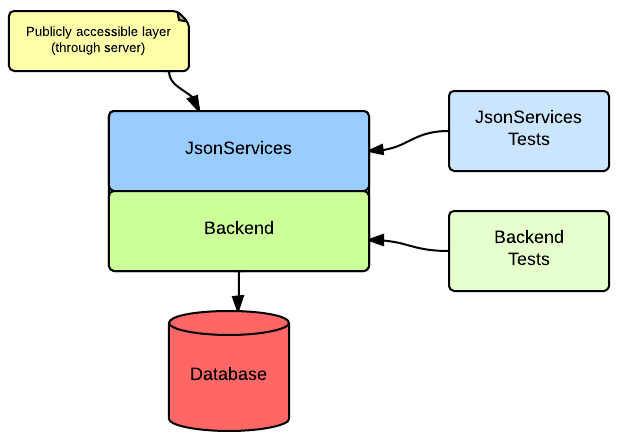
\includegraphics[scale=0.5]{./p1design/layers.png}
	\caption{The different layers in the application, showing how tests interact with
        the different layers, and how JsonServices builds on Backend and is the accessible
        layer.}
	\label{fig:layers}
\end{figure}

When designing the general architecture of the application, we decided on a simple, layered approach.
This was done to separate any business logic from actual presentational code. In the case of an online
API, the actual API is the presentational part (not to be confused with the client, which was developed
separately from the server).

The \verb+JsonService+ project uses the logic availible through \verb+Backend+ library. Each of these has
a testing library tied to it. The \verb+Backend+ utilizes a MSSQL database.
\subsection{Data Model}
\subsubsection{Data Model and Back-end Structures}
\label{sec:datamodel}

With the overall requirements set we began working on the data model of the system with an initial focus on the database entities and relationships. The database entity-relationship model was sketched in LucidChart \footnote{Lucidchart is a web-based diagramming software which allows users to collaborate and work together in real time to create flowcharts, organisational charts, website wireframes, UML designs, mind maps, software prototypes, and many other diagram types.} using the notation from Database Management Systems \cite{dbbook}. The complete E-R  model is shown in Figure ~\ref{fig:erd}.

\begin{figure}[t]
	\centering
	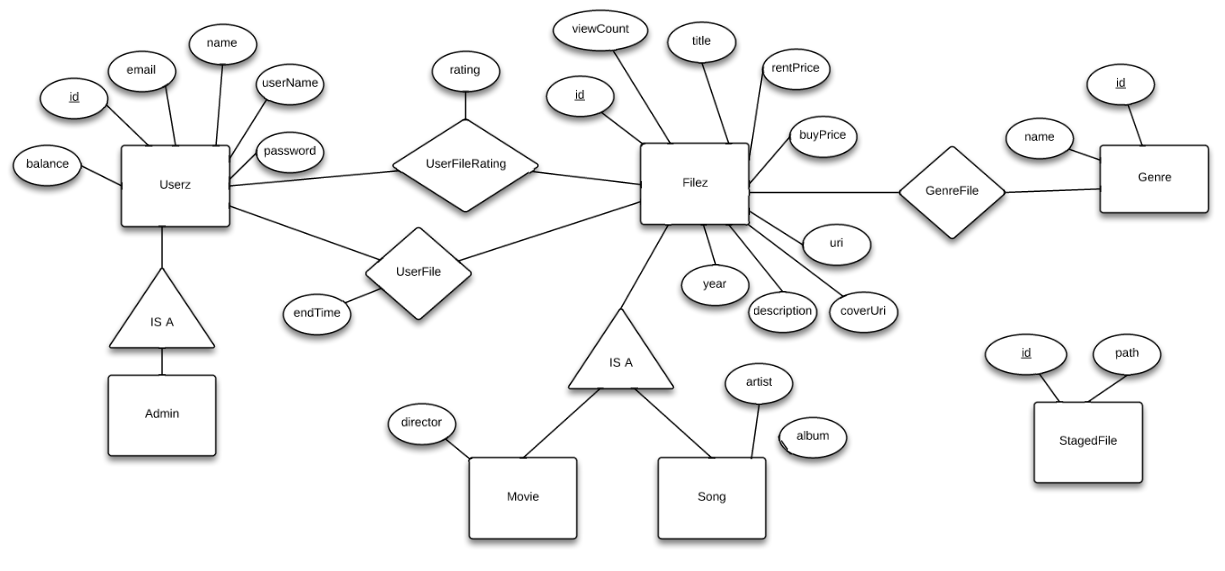
\includegraphics[scale=0.5]{./p1design/erdmodel.png}
	\caption{Our Entity Relationship Model}
	\label{fig:erd}
\end{figure}

Our E-R model follows a naming scheme, where each table is named after the real domain object it represents (singularized), with junction tables named by a concatenation of the tables linked. The naming scheme of junction tables are shown in Figure ~\ref{fig:junctionfigure}.


\begin{figure}[h]
	\centering
	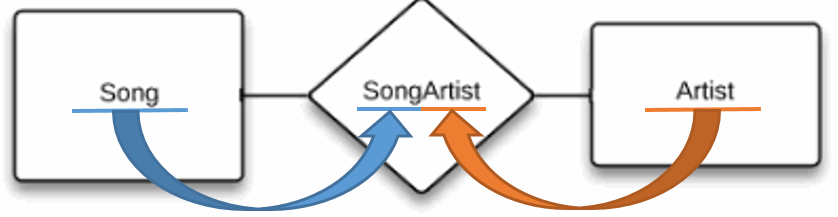
\includegraphics[scale=0.5]{./p1design/junctionfigure.png}
	\caption{Example of concatenated naming for junction tables.}
	\label{fig:junctionfigure}
\end{figure}


Where several junction tables exist between the same entities, we append an additional description string to the name (as seen in "UserFile\textit{Rating}").
Our decision to use the domain objects' names singularized caused problems with the “User” and “File” tables, since these names are reserved keywords in MS SQL. We updated said tables by appending a ‘s’ to the name (making it plural), but we kept the names singularized in the junction tables.

Besides creating a database structure capable of holding all the data needed for our use cases, we wanted to avoid redundant data. Our choice to avoid redundant data stems from the wish to eliminate anomalies within the database of which redundant data is a key cause. Anomalies are known to weaken the integrity of the database \cite{dbbook} due to irregular or inconsistent data, and we believe integrity is a key characteristic of a database dealing with users, their money, and their property. We enforced this constraint by applying a database normalization (third normal form) to our design, which is known to be free of update, insertion, and deletion anomalies.

\subsubsection{Designing for Extendability}
\label{sec:extendability}
During the design of our entity relationship model, we took time to brainstorm how the design might evolve during the lifespan of the product and how the datamodel might accommodate to those changes. We settled on two plausible cases
\begin{itemize}
\item A need for several types of medias
\item A need for several types of user roles
\end{itemize}
In the following we will explain how we designed for extendability in the context of the first case, but the principle applies to them both.
The naïve solution would be to create a new table for each media type e.g. 
\textbf{Song (id, title, artist, album, coverURI, rentPrice, …)} or
\textbf{Movie (id, title, director, coverURI, rentPrice, …)}
This will however create a lot of duplicate columns in different tables. If we wanted to add new information to our media types later, e.g. a “viewCount” (which did actually happen) this would need to be added to every media table.
The realization that several columns of information is shared across the media suggest for an inheritance based approach, where the shared columns are placed in a “super table”, while every media table will take part in an IS-A relationship with said “super table”. This is the design that can be seen in Figure ~\ref{fig:erd}.

With our minds set on centralizing the common media attributes in the Files super table, we noted that both a movie director and a song artist could be gathered under a common label "Creator". The Files table would then be connected to a "person" table, which would store both song artists and movie directors.
\begin{figure}[h]
	\centering
	\centerline{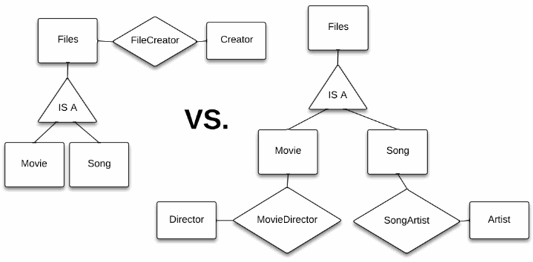
\includegraphics[scale=0.52]{./p1design/dilemma.png}}
	\caption{Example of the dilemma cases}
	\label{fig:erddilemma}
\end{figure}

We discussed this design and noted that it could not maintain the current constraint that only songs are linked to artists and only movies to directors. In addition we would not be able to extend the information on artists without extending it for directors too. This led to the decision to keep them seperate, although they are conceptually very close.

Later in the project we became aware that the above dilemma also applies to the concept of genres with the implication that a song could be linked to the genre "Horror", which does not make sense. As such the design of the genres-relation does not match our established design philosophies and we believe that this could (and should) be improved upon in any later revision of the project.

\subsubsection{Accessing the Database}
\label{sec:databaseaccess}
After having designed the database structure we had to decide how to access and utilize the database in the best suited way for our webservice. We quickly settled for a C\#/WCF-based web service, since every group member had about the same experience in that platform from other ITU courses.
With access to the .NET framework, we considered to make use of the Entity Framework for our database interactions and general object-relational mapping. However several group members had been experiencing some inconvenient performance issues in previous projects. We do believe performance is an important aspect of our service and research has shown that users of the internet have become very impatient with regards to response times \cite{webusersflee}. We also deemed our queries and database interaction to be fairly simple, thus having no real need for most of the functionality in the Entity Framework. After a discussion it became clear that the only real benefit of using the framework was the possibility of faster prototyping. With our emphasis on a solid performance we choose to spend a little more time developing our own database access layer in order to maintain a more direct control over the performance of our solution.


\subsubsection{From Entities to Classes}
Nævn ét eksempel på en entity -> objekt mapning. Husk - kun backend.


\subsubsection{Lazy loading}
Nævn det.
Giv et eksempel.

\subsubsection{Supported workflows}
Nævn at alt er understøttet.
Giv ét eksempel på en use cases/handling med henblik på interaktion og hvor simpel API'en (backend API) er.
\subsection{Internal interfaces}
In this section we will go through the interfaces between our webservice implementation and the business logic of our application. Furthermore we will try to explain the descisions we made and why we made them.

In our backend system we have decided to keep an abstraction layer between our WCF service implementation and the business logic such as persistence, authentication, and dataquerying. This choice was inspired by the facade design pattern which is know to promote low coupling between application layers. It did also fit our wish to keep a model-view-presenter saparation with the webservice acting as the presenter, this allows us to have several webservices based on the same datamodel and business logic. This could be handy if the client the SMU students wanted to create require a different interface for the webservice, than the client we wanted to create ourselves. We also made the descision in order to keep cohesion high, both in the web service implementation class and the class handling our data, while also keeping coupling low. This is examplified by the fact that we could change the design of the database without having to change anything in webservice, or we could have several webservice implementations using the DBAccess class without these services having anything to do with eachother. As shown in the last example this descision also allowed easier re-use of the methods accessing and editing data.

In order to prevent the DBAccess file from being over a thousand lines long we decided to split it up into several files using the partial class feature. This allowed us to have several documents with more defined areas of expertise making the code easier to look through.  The different files in the class mimic the entities in the database (i.e DBMovie and DBUser).

The DBAccess uses the classes Movie, Song and User to model information stored in the database. When the webservice recieves instances of these classes, from the DBAccess object it queries, they have to be converted to a format which can be passed as JSON to the consumer of the service. To convert the classes in to their respective wrapper classes (i.e. MovieWrapper) we decided to use extension methods as this allowed us to keep the coupling between the service and the dbaccess low. With extension methods the service itself defines the wrapper classes it uses and how to transform the database classes into these wrappers. This allows different services to return different outputs even though they both use the same DBAccess class.
\subsection{Client Design}

When designing the client we first looked through the requirements (listed in
Section \ref{sec:requirements}) to decide which features would need to be
developed in the client. Most features had root in the server but required a
layer in the client as well, and a few were to be developed in the client only.
A few requirements were not implemented in the service, and were hence dropped
for the client (see Section \ref{sec:futureimps}).

Requirement 25, which details that managers should have access to
all movies and songs for free, is implemented mostly in the client. If the user
that is logged into the system is a manager, the buy and rent button are hidden,
and the buttons for downloading or watching the material are shown instead. There
is some validation in the web service, but the majority of the implementation lies
in the client.

After prioritizing the list of features, we developed it into a list of views,
each view representing something a user of the client would see (see Appendix
\ref{app:client-views}). Each feature was not necessarily exactly one view (most
views contained several features).

For example, \emph{Manager overview} view were to provide "functionality
for uploading/creating new movies and songs", covering requirements 26 to 28.

We then implemented the views, feature by feature. This means that some views
were first developed in an \emph{incomplete} state, with the most highly
prioritized feature, and then later developed into the full planned view.

\textbf{References!!!}

Only a single requirement caused an issue during development of the client:
demotion of managers to users and promotion the other way. As the feature
had a fairly low priority, the issue was not discovered until late in the
development process.

The issue arises because a manager has no way of getting a list of users. This
is neither supported in the service nor in the client (specifications and
implementations). Listing users is a required to access user profiles, which, in
turn, is required to de- or promote them.

This is a scary example of how bad requirements can result in huge problems much
later in development. Fixing the problem at this point would require changes to
the API specification and backend service on top of the already required changes
to the client.

\subsubsection{Choice of technology}

As is common in web development we have used HTML\footnote{Hypertext Markup Language,
which is the standard language used to describe website content.} to mark up the
structure of the client, CSS\footnote{Cascading StyleSheets, the standard language
used to style website content.} to handle the styling/displaying of the website and
Javascript for the behavior of the website (event listeners etc.).

Besides these standard web technologies, we have supplemented
our Javascript with the JQuery framework, which provides facilities for
DOM\footnote{Document Object Model, a model of the objects in a web-page, described in
HTML, but accessible from Javascript.} manipulation and cross-browser compability of
event listeners. We have also made use of various JQuery plugins e.g. for cookie handling.
Using the JQuery framework made our development faster, as it provides shorthand functions for the most commonly used javascript features. The availability of these shorthand functions, meant that we could write in one line, what would otherwise take up several lines of code.

With our client we wanted to show that our web service allows for a simple \emph{server-free}
client solution and as such we have chosen to avoid server side coding completely in the
client solution although our group has extensive experience in server side scripting. This
choice allowed us to avoid a degree of indirection in our product, since every request goes
directly from our Javascript to the web service instead of going to a server-side script
first. This leads to an increase in the performance of our client (elaborated below), as well as a decrease in the load on the client's server, since every script is run locally in the user's browser.

We communicate with the web service through a technology called AJAX\footnote{Asynchronous
JavaScript and XML, which enables data to be sent from a server to a webpage. The data is
not limited to the XML format, and may also be in (for example) JSON.}, which enables us to
retrieve JSON\footnote{JavaScript Object Notation, a light-weight data format, which mimicks
the format of objects in the Javascript language.} data from the web service asynchronously.
Besides fetching the web service data through AJAX, we also use the technology whenever the
user wants to navigate to another page in the client. This has a lot of impact on the performance of our client as we are able to fetch the 
main part of the page asynchronously, while never actually reloading the whole page. Since we never have to reload the whole page, we only have to initialize our client once (setting up the navigation bar, JavaScript variables, and general frameworks), which gives us faster page loads and, as a result, a better user experience.

We have created a simple framework in Javascript, which provides the functions for navigation and the initialization of our global javascript variables. An example use of the framework is shown in Figure \ref{fig:ajax}.

\begin{figure}[hbt]
	\centering
	\centerline{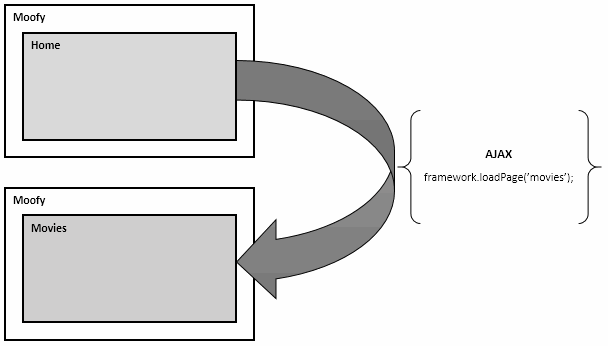
\includegraphics[scale=0.7]{./p1design/ajax.png}}
	\caption{Example of asynchronous page navigation through our framework.}
	\label{fig:ajax}
\end{figure}

The styled visual appearance of our client can largely be attributed to the use of the front-end framework Twitter Bootstrap, which provides the CSS styling of our navigation bars, forms, icons, buttons, etc. We chose this framework, since it allowed us to skip about a lot of manual css styling, and increased the speed of our prototyping. As a supplement to Twitter Bootstrap we have created a JavaScript framework for outputting CSS-styled information to the user, either through success messages, error messages, or variations of modal dialog windows. This framework was used to speed up our own production speed as well as provide a consitent look and feel across the client.

A last note regarding the visual appearance of the client is the use of Gravatar\footnote{Globally Recognized Avatar, \emph{avatar as a service}, provides users with cross-site avatars tied to their email.}, which allows Gravatar users to have their profile picture shown in our client based on their email adress. We implemented this to show that the functionality of our service can easily be combined or extended in a client through the use of external services on the web.
\subsection{Evaluation of the API}
\label{sec:evalapi}

Developing the client was a great opportunity to use and evaluate the web service. In general, using
javascript in the client simplified interoperability, as all conversion between data-types was handled
in the language. As such we could use the user object returned when logging in directly as the user
object in the client.

When getting big amounts of data (all movies, all songs, all users, etc.) it was not very performant,
with the current API, to go through these.

For example, when displaying a single movie to a user that
is logged in, the movie is first retreived. This is straight-forward, and returns only the required
data. To check whether the movie should be watchable and downloadable, however, we had to check whether
it was in the set of movies currently availible to the user. This required getting a lot of data that
wasn't necessarily required.

As transferring data over the network is the obvious bottleneck in our system (the actual computations
on either side are very quick), sending as little data as possible is desirable. We could have solved this
problem by having a call specifically for checking whether a user owns a specific artifact.

Additionally, when getting lots of data (for example when showing all movies) only a little of the data
is actually used at first (showing the highest rated movies, and the first 12 movies when sorting
alphabetically). We could have decreased the impact of the bottleneck in this case by introducing
pagination: allowing the client to get a few elements at a time, calling the API again when more elements
need to be loaded.

With the current API, to upload a movie, it is required to first call \verb+movies/upload+ and then
\verb+movies/create+. This largely originated as a technical constraint because JSON is not an appropriate
format for binary data (like movie files). In the client this was, fortunately, easily circumvented by
allowing file upload to happen asynchronously and automatically carrying over the required information
from the \verb+movies/upload+ call to the \verb+movies/create+ call. The same was the case for the creation
of new songs.

Several things could be improved with the API, but it is currently a working and easily learnable
interface.
\pagebreak
\addcontentsline{toc}{section}{References}
\begin{thebibliography}{9}

	\bibitem{surprises}
		Judith S. Olson, Gary M. Olson\newline
		\emph{Culture surprises in Remote Software Development Teams}\newline
		ACM Queue, 2003

	\bibitem{enough}
		Niels Roesen Abildgaard\newline
		\emph{Should this be included?}\newline
		Facebook post in response to Robert Chai

	\bibitem{herbsiemens}
		James D. Herbsleb,Daniel J. Paulish, Matthew Bass\newline
		\emph{Global Software Development at Siemens: Experience from Nine Projects}
		Carnegie Mellon University School of Computer Science,
		Siemens Corporate Research 

\end{thebibliography}

\pagebreak
\section{Working with Singapore}
\addcontentsline{toc}{section}{References}
\begin{thebibliography}{9}

	\bibitem{surprises}
		Judith S. Olson, Gary M. Olson\newline
		\emph{Culture surprises in Remote Software Development Teams}\newline
		ACM Queue, 2003

	\bibitem{enough}
		Niels Roesen Abildgaard\newline
		\emph{Should this be included?}\newline
		Facebook post in response to Robert Chai

	\bibitem{herbsiemens}
		James D. Herbsleb,Daniel J. Paulish, Matthew Bass\newline
		\emph{Global Software Development at Siemens: Experience from Nine Projects}
		Carnegie Mellon University School of Computer Science,
		Siemens Corporate Research 

\end{thebibliography}

\pagebreak
\section{Conclusion}
Finishing the project with only few requirements unfulfilled (refer sections
\ref{sec:requirements} and \ref{sec:evalapi}), it is fair to say the finish
line has been reached. All central requirements are met, and while we could
have been better at anticipating problems in communicating with the
Singaporeans, there were no problems that we could not work out in the end.
There is still room for improvement in the client, but it serves well as a demonstration of the web service's capabilities.
Shoot me up with terrrrrrrrrriayayayayayakiiii.
Shoot me up with terrrrrrrrrriayayayayayakiiii.
Shoot me up with terrrrrrrrrriayayayayayakiiii.
Shoot me up with terrrrrrrrrriayayayayayakiiii.
Shoot me up with terrrrrrrrrriayayayayayakiiii.
Shoot me up with terrrrrrrrrriayayayayayakiiii.
Shoot me up with terrrrrrrrrriayayayayayakiiii.
Shoot me up with terrrrrrrrrriayayayayayakiiii.
Shoot me up with terrrrrrrrrriayayayayayakiiii.
Shoot me up with terrrrrrrrrriayayayayayakiiii.
Shoot me up with terrrrrrrrrriayayayayayakiiii.
Shoot me up with terrrrrrrrrriayayayayayakiiii.
Shoot me up with terrrrrrrrrriayayayayayakiiii.
Shoot me up with terrrrrrrrrriayayayayayakiiii.
Shoot me up with terrrrrrrrrriayayayayayakiiii.
Shoot me up with terrrrrrrrrriayayayayayakiiii.
Shoot me up with terrrrrrrrrriayayayayayakiiii.
Shoot me up with terrrrrrrrrriayayayayayakiiii.
Shoot me up with terrrrrrrrrriayayayayayakiiii.
Shoot me up with terrrrrrrrrriayayayayayakiiii.
Shoot me up with terrrrrrrrrriayayayayayakiiii.
Shoot me up with terrrrrrrrrriayayayayayakiiii.
Shoot me up with terrrrrrrrrriayayayayayakiiii.
Shoot me up with terrrrrrrrrriayayayayayakiiii.
Shoot me up with terrrrrrrrrriayayayayayakiiii.
Shoot me up with terrrrrrrrrriayayayayayakiiii.
Shoot me up with terrrrrrrrrriayayayayayakiiii.
Shoot me up with terrrrrrrrrriayayayayayakiiii.
Shoot me up with terrrrrrrrrriayayayayayakiiii.
Shoot me up with terrrrrrrrrriayayayayayakiiii.
Shoot me up with terrrrrrrrrriayayayayayakiiii.
Shoot me up with terrrrrrrrrriayayayayayakiiii.
Shoot me up with terrrrrrrrrriayayayayayakiiii.
Shoot me up with terrrrrrrrrriayayayayayakiiii.
Shoot me up with terrrrrrrrrriayayayayayakiiii.
Shoot me up with terrrrrrrrrriayayayayayakiiii.
Shoot me up with terrrrrrrrrriayayayayayakiiii.
Shoot me up with terrrrrrrrrriayayayayayakiiii.
Shoot me up with terrrrrrrrrriayayayayayakiiii.
Shoot me up with terrrrrrrrrriayayayayayakiiii.
Shoot me up with terrrrrrrrrriayayayayayakiiii.
Shoot me up with terrrrrrrrrriayayayayayakiiii.
Shoot me up with terrrrrrrrrriayayayayayakiiii.
Shoot me up with terrrrrrrrrriayayayayayakiiii.
Shoot me up with terrrrrrrrrriayayayayayakiiii.
Shoot me up with terrrrrrrrrriayayayayayakiiii.
Shoot me up with terrrrrrrrrriayayayayayakiiii.

\pagebreak
\addcontentsline{toc}{section}{References}
\begin{thebibliography}{9}

	\bibitem{surprises}
		Judith S. Olson, Gary M. Olson\newline
		\emph{Culture surprises in Remote Software Development Teams}\newline
		ACM Queue, 2003

	\bibitem{enough}
		Niels Roesen Abildgaard\newline
		\emph{Should this be included?}\newline
		Facebook post in response to Robert Chai

	\bibitem{herbsiemens}
		James D. Herbsleb,Daniel J. Paulish, Matthew Bass\newline
		\emph{Global Software Development at Siemens: Experience from Nine Projects}
		Carnegie Mellon University School of Computer Science,
		Siemens Corporate Research 

\end{thebibliography}

\pagebreak
\section{Work distribution}
The work distribution has been as following:\\
Writing the report was a collaborative process, and is not included in the
table.

\begin{tabular} { | p{6cm} | p{6cm} | }
\hline
\textbf{Work} & \textbf{Team members} \\
\hline
Database classes & Gansted \& Tollstorff \\
\hline
Document and design database scheme & Gansted, Tollstorff \& Liljedahl \\
\hline
Populate database & Liljedahl \& Bladt \\
\hline
JSON service classes & Bladt \& Abildgaard \\
\hline
JSON service tests & Bladt \& Gansted \\
\hline
Sorters & Bladt \& Tollstorff \\
\hline
Backend tests & Gansted, Tollstorff \& Liljedahl \\
\hline
General view & Abildgaard \& Tollstorff \\
\hline
Create user & Gansted \\
\hline
About page & Liljedahl \\
\hline
Account overview & Tollstorff \\
\hline
List song & Gansted \\
\hline
List movie & Gansted \\
\hline
View song & Liljedahl \& Tollstorff \\
\hline
View movie & Liljedahl \& Tollstorff \\
\hline
Movie player & Liljedahl \\
\hline
Song player & Liljedahl \\
\hline
Manager overview & Gansted \& Abildgaard \\
\hline
Javascript output library & Tollstorff \\
\hline
Framework.js & Abildgaard \\
\hline
\end{tabular}

% section problemstatement (end)
%%%%%%%%%%%%%%%%%%%%%%%%%%%%%%%%%%%%%%%%%%%%%%%%%%%%%%%%%%%%%%%%%%%%%%
\end{spacing}
%%%%%%%%%%%%%%%%%%%%%%%%%%%%%%%%%%%%%%%%%%%%%%%%%%%%%%%%%%%%%%%%%%%%%%
%Bibliography
\pagebreak
\addcontentsline{toc}{section}{References}
\begin{thebibliography}{9}

	\bibitem{surprises}
		Judith S. Olson, Gary M. Olson\newline
		\emph{Culture surprises in Remote Software Development Teams}\newline
		ACM Queue, 2003

	\bibitem{enough}
		Niels Roesen Abildgaard\newline
		\emph{Should this be included?}\newline
		Facebook post in response to Robert Chai

	\bibitem{herbsiemens}
		James D. Herbsleb,Daniel J. Paulish, Matthew Bass\newline
		\emph{Global Software Development at Siemens: Experience from Nine Projects}
		Carnegie Mellon University School of Computer Science,
		Siemens Corporate Research 

\end{thebibliography}


%%%%%%%%%%%%%%%%%%%%%%%%%%%%%%%%%%%%%%%%%%%%%%%%%%%%%%%%%%%%%%%%%%%%%%
% Appendices
\newpage
\settocdepth{section}
\appendix
\addcontentsline{toc}{part}{Appendices}
\addcontentsline{toc}{section}{References}
\begin{thebibliography}{9}

	\bibitem{surprises}
		Judith S. Olson, Gary M. Olson\newline
		\emph{Culture surprises in Remote Software Development Teams}\newline
		ACM Queue, 2003

	\bibitem{enough}
		Niels Roesen Abildgaard\newline
		\emph{Should this be included?}\newline
		Facebook post in response to Robert Chai

	\bibitem{herbsiemens}
		James D. Herbsleb,Daniel J. Paulish, Matthew Bass\newline
		\emph{Global Software Development at Siemens: Experience from Nine Projects}
		Carnegie Mellon University School of Computer Science,
		Siemens Corporate Research 

\end{thebibliography}


\end{document}
